% THIS IS SIGPROC-SP.TEX - VERSION 3.1
% WORKS WITH V3.2SP OF ACM_PROC_ARTICLE-SP.CLS
% APRIL 2009
%
% It is an example file showing how to use the 'acm_proc_article-sp.cls' V3.2SP
% LaTeX2e document class file for Conference Proceedings submissions.
% ----------------------------------------------------------------------------------------------------------------
% This .tex file (and associated .cls V3.2SP) *DOES NOT* produce:
%       1) The Permission Statement
%       2) The Conference (location) Info information
%       3) The Copyright Line with ACM data
%       4) Page numbering
% ---------------------------------------------------------------------------------------------------------------
% It is an example which *does* use the .bib file (from which the .bbl file
% is produced).
% REMEMBER HOWEVER: After having produced the .bbl file,
% and prior to final submission,
% you need to 'insert'  your .bbl file into your source .tex file so as to provide
% ONE 'self-contained' source file.
%
% Questions regarding SIGS should be sent to
% Adrienne Griscti ---> griscti@acm.org
%
% Questions/suggestions regarding the guidelines, .tex and .cls files, etc. to
% Gerald Murray ---> murray@hq.acm.org
%
% For tracking purposes - this is V3.1SP - APRIL 2009

\documentclass{sig-alternate}

\newfont{\mycrnotice}{ptmr8t at 7pt}
\newfont{\myconfname}{ptmri8t at 7pt}
\let\crnotice\mycrnotice%
\let\confname\myconfname%

\permission{Permission to make digital or hard copies of part or all of this work for personal or classroom use is granted without fee provided that copies are not made or distributed for profit or commercial advantage and that copies bear this notice and the full citation on the first page. Copyrights for third-party components of this work must be honored. For all other uses, contact the Owner/Author. \\ Copyright is held by the owner/author(s).}
\conferenceinfo{SIGMOD'15,}{May 31--June 4, 2015, Melbourne, Victoria, Australia.} 
\copyrightetc{ACM \the\acmcopyr}
\crdata{978-1-4503-2758-9/15/05. \\
http://dx.doi.org/10.1145/2723372.2742787}

\clubpenalty=10000 
\widowpenalty = 10000

\usepackage{url}
\usepackage{algorithmic}
\usepackage{algorithm}
\usepackage{listings}
\usepackage{balance}
\usepackage{xfrac}
\usepackage{multirow}
\lstdefinelanguage{scala}{morekeywords={class,object,trait,extends,with,new,if,while,for,def,val,var,this},
otherkeywords={->,=>},
sensitive=true,
morecomment=[l]{//},
morecomment=[s]{/*}{*/},
morestring=[b]"}
% Default settings for code listings
\lstset{frame=tb,language=scala,aboveskip=3mm,belowskip=3mm,showstringspaces=false,columns=flexible,basicstyle={\small\ttfamily}}

\begin{document}

\title{Rethinking Data-Intensive Science Using \linebreak Scalable Analytics Systems}
%
% You need the command \numberofauthors to handle the 'placement
% and alignment' of the authors beneath the title.
%
% For aesthetic reasons, we recommend 'three authors at a time'
% i.e. three 'name/affiliation blocks' be placed beneath the title.
%
% NOTE: You are NOT restricted in how many 'rows' of
% "name/affiliations" may appear. We just ask that you restrict
% the number of 'columns' to three.
%
% Because of the available 'opening page real-estate'
% we ask you to refrain from putting more than six authors
% (two rows with three columns) beneath the article title.
% More than six makes the first-page appear very cluttered indeed.
%
% Use the \alignauthor commands to handle the names
% and affiliations for an 'aesthetic maximum' of six authors.
% Add names, affiliations, addresses for
% the seventh etc. author(s) as the argument for the
% \additionalauthors command.
% These 'additional authors' will be output/set for you
% without further effort on your part as the last section in
% the body of your article BEFORE References or any Appendices.

%  in this sample file, there are a *total*
% of EIGHT authors. SIX appear on the 'first-page' (for formatting
% reasons) and the remaining two appear in the \additionalauthors section.
%
\numberofauthors{1} 
\author{\alignauthor Frank~Austin~Nothaft$^{*}$, Matt~Massie$^{*}$, Timothy~Danford$^{*,\ddagger}$, Zhao~Zhang$^{*}$, Uri~Laserson$^{\circ}$, Carl~Yeksigian$^{\ddagger}$, Jey~Kottalam$^{*}$, Arun~Ahuja$^{\dagger}$, Jeff~Hammerbacher$^{\dagger, \circ}$, Michael~Linderman$^{\dagger}$, Michael~J.~Franklin$^{*}$, Anthony~D.~Joseph$^{*}$, David~A.~Patterson$^{*}$ \\
$^{*}$\affaddr{AMPLab, University of California, Berkeley}, $^{\circ}$\affaddr{Cloudera, San Francisco, CA} \\
$^{\dagger}$\affaddr{Carl Icahn School of Medicine, Mount Sinai, New York, NY},
$^{\ddagger}$\affaddr{Genomebridge, Cambridge, MA} \\
\email{\{fnothaft, massie, tdanford, zhaozhang, jey, franklin, adj, pattrsn\}@berkeley.edu} \\
\email{\{arun.ahuja, jeff.hammerbacher, michael.linderman\}@mssm.edu} \\
\email{laserson@cloudera.com} \email{cyeksig@genomebridge.org} \\
} 
% You can go ahead and credit any number of authors here,
% e.g. one 'row of three' or two rows (consisting of one row of three
% and a second row of one, two or three).
%
% The command \alignauthor (no curly braces needed) should
% precede each author name, affiliation/snail-mail address and
% e-mail address. Additionally, tag each line of
% affiliation/address with \affaddr, and tag the
% e-mail address with \email.
%
% 1st. author% There's nothing stopping you putting the seventh, eighth, etc.
% author on the opening page (as the 'third row') but we ask,
% for aesthetic reasons that you place these 'additional authors'
% in the \additional authors block, viz.

% Just remember to make sure that the TOTAL number of authors
% is the number that will appear on the first page PLUS the
% number that will appear in the \additionalauthors section.

\maketitle

\begin{abstract}
``Next generation'' data acquisition technologies are allowing scientists to collect exponentially more data at a
lower cost. These trends are broadly impacting many scientific fields, including genomics, astronomy, and
neuroscience. We can attack the problem caused by exponential data growth by applying horizontally scalable
techniques from current analytics systems to accelerate scientific processing pipelines.

In this paper, we describe \texttt{ADAM}, an example genomics pipeline that leverages the open-source Apache
\texttt{Spark} and \texttt{Parquet} systems to achieve a $28\times$ speedup over current genomics
pipelines, while reducing cost by 63\%. From building this system, we were able to distill a set of techniques for
implementing scientific analyses efficiently using commodity ``big data'' systems. To demonstrate the generality of our
architecture, we then implement a scalable astronomy image processing system which achieves a 2.8--$8.9\times$
improvement over the state-of-the-art MPI-based system.
\end{abstract}

% A category with the (minimum) three required fields
\category{L.4.1}{Applied Computing}{Life and medical sciences}[Computational biology]
\category{H.1.3.2}{Information Systems}{Data management systems}[Database management
system engines, parallel and distributed DBMSs]
\category{E.3.2}{Software and its Engineering}{Software creation and management}[Software
Development Process Management]

\terms{Design}

\keywords{Analytics, MapReduce, Genomics, Scientific Computing}

\section{Introduction}
\label{sec:introduction}

Major improvements in scientific data acquisition techniques are driving increased scientific data storage and
processing needs~\cite{cunningham14, schadt10}. In fields like
neuroscience~\cite{freeman14} and \linebreak genomics~\cite{stein10}, particle physics, and astronomy,
scientists routinely perform analyses that process terabytes~(TB) to \linebreak petabytes~(PB) of data.
While traditional scientific computing and storage platforms are optimized for fast linear algebra, many emerging
domains make heavy use of statistical learning techniques and user defined functions~(UDFs) on top of
semistructured data. This move towards statistical techniques has been driven by the increase in the
amount of data available to scientists. At the same time, commercial needs have led to the development of
horizontally-scalable analytics systems like \texttt{MapReduce}~\cite{dean04, dean08} and
\texttt{Spark}~\cite{zaharia10}, as well as statistical systems that are accessible to non-experts, such as
\texttt{Scikit-learn}~\cite{pedregosa11} and \texttt{MLI}~\cite{sparks13}.

Since the amount of scientific data being generated is growing so quickly, there is a good opportunity to apply
modern, horizontally scalable analytics systems to science. New scientific
projects such as the 100K for UK, which aims to sequence the genomes of 100,000 individuals in the
United Kingdom~\cite{uk100k} will generate three to four orders of magnitude more data than
prior projects like the 1000 Genomes Project~\cite{siva08}. These projects use the current ``best
practice'' genomic variant calling pipeline~\cite{auwera13}, which takes approximately 120 hours to
process a single, high-quality human genome using a single, beefy node~\cite{talwalkar14}. To address
these challenges, scientists have started to implement computer systems techniques such as
map-reduce~\cite{mckenna10} and columnar storage~\cite{fritz11} in custom
scientific compute/storage systems. While these systems have improved analysis cost and performance,
current implementations incur significant overheads imposed by the legacy formats and
codebases that they use.

In this paper, we demonstrate \texttt{ADAM}~\cite{massie13}, a genomic data processing system built using Apache
\texttt{Avro}, \texttt{Parquet}, and \texttt{Spark}~\cite{avro, parquet, zaharia10}, that achieves a 28$\times$
increase in read preprocessing throughput over the current best
practice pipeline, while reducing analysis cost by 63\%. In the process of creating this
system, we developed a ``narrow waisted'' layering model for building similar scientific analysis systems.
This narrow waisted stack is inspired by the OSI model for networked systems~\cite{zimmermann80}. Our model
uses the data schema as the narrow waist that separates data processing from data storage. \texttt{ADAM} additionally
demonstrates that it is possible to achieve very high performance on scientific applications using free open source
software~(OSS). By shifting scientific data processing away from proprietary high performance computing~(HPC)
environment and into a commodity/OSS world, we can democratize scientific analysis.

To researchers and practitioners unfamiliar with current practice in computational science, the layering-based approach
we propose may appear sufficiently straightforward as to be uncontroversial. In practice however---as discussed in the
seminal ``end-to-end'' paper~\cite{saltzer84}---there is a common tendency to engage in ``stack smashing'' when building
a large system to improve performance or to simplify implementation. Scientific applications are no different; in genomics,
processing pipelines impose invariants on the layout of data on disk to improve performance, such as requiring data to be
stored in a coordinate-sorted order. These invariants are rarely made explicit, which can lead to functional errors when
composing multiple tools into a pipeline and necessitate slow sorting stages. In both genomics and astronomy, data is
stored in flat file that centralize file/experiment metadata in order to improve the size of data on disk. This increases the
cost of parallel metadata access and limits the scalability of current parallel astronomy pipelines
(see~\S\ref{sec:astro-workloads}). In this paper, we demonstrate that scientific pipelines \emph{can} be decomposed
without sacrificing computational cost through the use of the following techniques:

\begin{enumerate}
\item We make the schema the ``narrow waist'' of our stack and enforce data independence. We then
devise algorithms for making common scientific processing patterns fast (e.g., coordinate-space joins,
see~\S\ref{sec:coordinate-system-joins}).
\item To improve horizontal scalability, we push computation to the data. To support this, we use \texttt{Parquet}, a
modern parallel columnar store based off of \texttt{Dremel}~\cite{melnik10}.
\item We use a denormalized schema to achieve O(1) parallel access to metadata.
\end{enumerate}

\begin{figure}[h]
\begin{center}
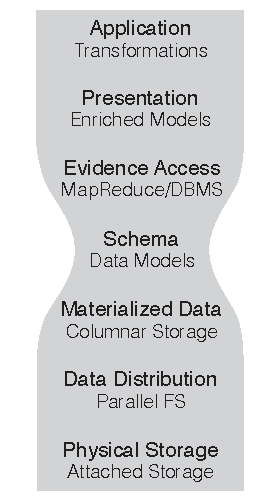
\includegraphics{stack-model-2.pdf}
\end{center}
\caption{A stack model for scientific computing}
\label{fig:stack-model}
\end{figure}

We introduce the stack model in Figure~\ref{fig:stack-model} as a way to decompose scientific systems. In
addition to the genomics application described above, we demonstrate the generality of this model by using it to
implement a system for processing astronomy images and achieve a 2.8--$8.9\times$ performance
improvement over a state-of-the-art Message Passing Interface~(MPI) based pipeline.

While the stack smashing used in genomics to accelerate common access patterns is undesirable because it
violates data independence and can lead to errors when composing multiple tools into a pipeline, we also find
that it can lead to correctness errors inside of a single tool. As noted
above, tools built using the current Sequence/Binary Alignment and Map~(\texttt{SAM}/\texttt{BAM}~\cite{li09}) formats
for storing genomic alignments apply constraints about record ordering to enable specific computing patterns. Our
implementation~(described in~\S\ref{sec:genomics-pipeline}) identifies errors in two current genomics
processing stages that occur \emph{because} of the sorted data layout invariant. Our implementations of
these stages do not make use of sort order, and achieve high performance while eliminating these errors.

We have made all of the software~(source code and executables) described in this paper available free
of charge under the permissive Apache 2 open-source license. Additionally, the setup for implementing the
genomics experiments described in this paper has been made publicly available to enable reproducing our
results. Access instructions are given in Appendices~\ref{sec:availability} and \ref{sec:experimental-setup}.

\section{Background}
\label{sec:background}

Our work is at the intersection of computational science, data management, and processing
systems. Our architectural approach is informed by recent trends in both areas. The design of
large scale data management has changed dramatically since the papers by Dean and
Ghemawat~\cite{dean04, dean08} that described Google's \texttt{MapReduce} system. Over a
similar timeframe, scientific fields have taken advantage of improvements in data acquisition
technologies. Since the Human Genome Project finished in 2001~\cite{lander01}, the price
of genomic sequencing has dropped by 10,000$\times$~\cite{nhgri}. This drop in cost has enabled the
capture of petabytes of sequence data and enabled significant population genomics
experiments like the 1000 Genomes project~\cite{siva08} and The Cancer Genome Atlas~(TCGA,
\cite{weinstein13}). These changes are not unique to genomics; indeed, fields such as
neuroscience~\cite{cunningham14} and astronomy~\cite{lsst2008, turk11, sdss2000} are experiencing similar
trends.

Although there has been significant progress in the development of systems for processing large
datasets---the development of first generation map-reduce systems~\cite{dean04}, followed by
iterative map-reduce systems like \texttt{Spark}~\cite{zaharia10}, as well as parallel and columnar
DBMS~\cite{abadi06, lamb12}---the uptake of these systems in the scientific world has been slow.
Most implementations have either used map-reduce as an inspiration for API
design~\cite{mckenna10}, or have been systems that have used map-reduce to
parallelize existing toolkits~\cite{langmead09, schatz09}. These approaches are perilous for several
reasons:

\begin{itemize}
\item A strong criticism of the map-reduce model is that the API is insufficiently expressive
for describing complex tasks. As a consequence of this, tools like the \texttt{GATK}~\cite{mckenna10} that
adopt map-reduce as a programming model force significant restrictions on algorithm implementors. For
example, a \texttt{GATK walker} is provided with a single view over the data~(a sorted iterator) with limited reduce
functionality.
\item A major contribution of systems like \texttt{MapReduce}~\cite{dean08} and \texttt{Spark}~\cite{zaharia10,
zaharia12} is the ability to reliably distribute parallel tasks across a cluster in an automated fashion. While
the \texttt{GATK} uses map-reduce as a programming abstraction, it does not use map-reduce as an execution strategy.
To run tools like the \texttt{GATK} across a cluster, organizations use workflow management systems for sharding and
persisting intermediate data, and managing failures and retries. This \emph{ad hoc} approach is a source of inefficiency
during execution: since the execution system cannot pipeline jobs together, iterative stages in the \texttt{GATK} must
spill to disk and become bottlenecked by I/O performance.
\item The \texttt{Hadoop}-based implementations in \texttt{Crossbow}~\cite{langmead09} and
\texttt{Cloudburst}~\cite{schatz09} run unmodified legacy tools on top of \texttt{Hadoop}. This approach does
achieve speedups, but does not attack overhead. High overhead occurs due to duplicated loading of indices and poor
broadcast performance.
\end{itemize}

Recent work by Diao et al~\cite{diao15} has looked at optimizing map-reduce systems for
processing genomic data. They adapt strategies from the query optimization literature to reorder
computation to minimize data shuffling. While this approach does improve shuffle traffic, several
preprocessing stages cannot be transposed. For instance, reversing the order of realignment and
base quality score recalibration~(see~\S\ref{sec:genomics-pipeline}) will change the inferred quality
score distribution. Additionally, we believe that the shuffle traffic that Diao et al observe is an artifact
caused by the abstraction inversion discussed in~\S\ref{sec:introduction}. As we demonstrate
in~\S\ref{sec:genomics-pipeline}, these penalties can be eliminated by restructuring the pre-processing
algorithms.

One notable area where modern data management techniques have been leveraged by scientists is in
the data storage layer. Due to the storage costs of large genomic datasets, scientists have introduced the
\texttt{CRAM} format that uses columnar storage techniques and special compression algorithms to achieve a
$>30$\% reduction in size over the compressed \texttt{BAM} format~\cite{fritz11}. While \texttt{CRAM} achieves
high~($\gg 50\%$) compression, it imposes restrictions on the ordering and structure of the data, and does not provide
support for predicates or projection. Additionally, to achieve compression ratios greater than 30\%, \texttt{CRAM} uses
lossy compression codecs. We perform a more comprehensive comparison against \texttt{CRAM}
in~\S\ref{sec:column-store-perf}.

One interesting trend of note is the development of \linebreak databases specifically for scientific applications.
The exemplar is \texttt{SciDB}, which provides an array-driven storage model with efficient
linear algebra routines~\cite{brown10}. While arrays accelerate many linear algebra based routines, they
are not a universally great fit. Due to the semistructured nature of genomics datasets, complex UDFs are needed
to import genomic data into array databases. Other systems like the Genome Query Language~(\texttt{GQL},
\cite{kozanitis14}) have extended SQL to provide efficient query semantics across
genomic coordinates. While \texttt{GQL} achieves 10$\times$ performance improvements for certain
algorithms, SQL is not an attractive language for scientific analyses that make heavy use of UDFs.

\section{Characteristics of Scientific \\ Analysis Systems}
\label{sec:principles}

Most prior work on scientific computing has been focused on linear algebra and other problems that can
be structured as a matrix or network. However, in several of the emerging data-driven scientific
disciplines, data is less rigorously structured. As discussed in~\S\ref{sec:background}, scientists have
developed custom solutions to process this data. In this
section, we discuss the common characteristics of workloads in these emerging scientific areas. Given
these characteristics, we describe a way to decompose data processing and storage systems so that
we can efficiently implement important processing patterns while providing a wide range of data access
methods.

\subsection{Layering}
\label{sec:layering}

The processing patterns being applied to scientific data shift widely
as the data itself ages. Because of this change, we want to design a scientific data processing system that is
flexible enough to accommodate our different use cases. At the same time, we want to ensure that the
components in the system are well isolated so that we do not bleed functionality across the stack. If
we did bleed functionality across layers in the stack, this violation of the end-to-end principle would make it more
difficult to implement different applications using our stack~\cite{saltzer84}. Additionally, as we discuss
in~\S\ref{sec:genomics-pipeline}, improper separation of concerns can lead to errors in our application.

These concerns are very similar to the factors that led to the development of the Open Systems
Interconnection~(OSI) model and Internet Protocol~(IP) stack for networking
services~\cite{zimmermann80}. The networking stack models were designed to allow the mixing and
matching of different protocols, all of which existed at different functional levels. The success of the
networking stack model can largely be attributed to the ``narrow waist'' of the stack, which simplified the
integration of a new protocol or technology by ensuring that the protocol only needed to implement a
single interface to be compatible with the rest of the stack.

Unlike conventional scientific systems that leverage custom data formats like \texttt{BAM}, \texttt{SAM},
or \texttt{CRAM}~\cite{fritz11, li09}, we believe that the use of an explicit schema for data interchange is critical.
In our stack model shown in Figure~\ref{fig:stack-model}, the schema becomes the ``narrow waist''
of the stack. Most importantly, placing the schema as the narrow waist enforces a strict separation
between data storage/access and data processing. The seven layers of our stack model
are decomposed as follows, and are numbered in ascending order from bottom to top:

\begin{enumerate}
\item {\bf Physical Storage} coordinates data writes to physical media.
\item {\bf Data Distribution} manages access, replication, and distribution of the files that have
been written to storage media.
\item {\bf Materialized Data} encodes the patterns for how data is encoded and stored. This
layer determines I/O bandwidth and compression.
\item {\bf Data Schema} specifies the representation of data, and forms the narrow waist of
the stack that separates access from execution.
\item {\bf Evidence Access} provides primitives for processing data, and enables the transformation of
data into different views and traversals.
\item {\bf Presentation} enhances the data schema with convenience methods for performing
common tasks and accessing common derived fields from a single element.
\item {\bf Application}s use the evidence access and presentation layers to compose
algorithms for performing an analysis.
\end{enumerate}

A well defined software stack has several other significant advantages. By limiting application
interactions with layers lower than the presentation layer, application developers are given a clear and
consistent view of the data they are processing, and this view of the data is independent of whether the
data is local or distributed across a cluster or cloud. With careful design in the data format and data access layers,
we can seamlessly
support conventional whole file access patterns, while also allowing easy access to small slices of files.
By treating the compute substrate and storage as separate layers, we also drastically increase
the portability of the APIs that we implement.

As we discuss in more detail in~\S\ref{sec:genomics-pipeline}, current scientific systems bleed functionality between
stack layers. The \texttt{BAM}, \texttt{SAM} and \texttt{CRAM} formats are exemplars, as they expect data
to be sorted by genomic coordinate. This modifies the layout of data on disk~(level 3, Materialized Data)
and constrains how applications traverse datasets~(level 5, Evidence Access). Beyond
constraining applications, this leads to bugs in applications that are difficult to detect.\footnote{Current BQSR and
Duplicate Marking implementations fail in certain corner-case alignments, due to an improper sort order invariant.}
To resolve this conflict, we demonstrate several ways to efficiently implement conventional scientific
traversals without imposing a sort order invariant in~\S\ref{sec:optimizations-scientific-processing}. These traversals
are implemented above the evidence access layer, and are independent of anything below the schema.

The idea of decomposing scientific applications into a stack model is not new; Bafna et al~\cite{bafna13}
made a similar suggestion in 2013. We borrow some vocabulary from Bafna et al, but our approach is
differentiated in several critical ways:

\begin{itemize}
\item Bafna et al consider the stack model specifically in the context of data management systems for
genomics; as a result, they bake current technologies and design patterns into the stack. Instead, a stack
design should serve to abstract layers from methodologies/implementations, lest technology trends render
the stack obsolete.
\item Bafna et al define a binary data format as the narrow waist in their stack, instead of a schema.
While these two seem interchangeable, they are not in practice. A schema provides a view of the logical content
of data, while a binary data format provides a view of the physical layout of data.
\item Notably, Bafna et al use this stack model to motivate \texttt{GQL}~\cite{kozanitis14}. While a query system
should provide a way to process and transform data, Bafna et al instead move this system down to the
data materialization layer. We feel that this approach inverts the semantics that a user of \texttt{GQL} would expect.
\end{itemize}

Our stack enables us to serve the use cases we outline in~\S\ref{sec:workloads}. By using
\texttt{Parquet} as a storage format, we are able to process the data in many \texttt{Hadoop}-based systems. We
implement high performance batch and interactive processing with \texttt{Spark}, and can delegate to
systems like \texttt{Impala}~\cite{kornacker15} and \texttt{Spark SQL}~\cite{armbrust15} for data warehousing.

\subsection{Workloads}
\label{sec:workloads}

There are several common threads that unify the diverse set of applications that make up scientific
computing. When looking at the data that is used in different fields, several trends pop out:

\begin{enumerate}
\item Scientific data tends to be rigorously associated with coordinates in some domain. These coordinate
systems vary, but can include:
\begin{itemize}
\item Time~(e.g., fMRI data, particle simulations)
\item Chromosomal position~(e.g., genomic read alignments and variants)
\item Position in space~(imaging data, some \linebreak sensor datasets, see \texttt{Hadoop-GIS}~\cite{aji13} and
\texttt{SpatialHadoop}~\cite{eldawy15})
\end{itemize}
\item For aggregated data, we frequently want to slice data into many different views. For example, for time
domain data aggregated from many sensors, scientists may want to perform analyses by slicing
across a single point in time, or by slicing across a single sensor. In genomics, we frequently aggregate data
across many people from a given population. Once we have done this first aggregation, we may want to then
slice the data by subsets of the population, or by regions of the genome~(e.g., specific genes of interest).
\end{enumerate}

There are two important consequences of the characteristics above. First, since data is attached to a
coordinate system, the coordinate system itself may impose logical processing patterns. For example, for
time domain data, we may frequently need to run functions that pass a sliding window across the dataset (e.g., for
convolution). Second, the slicing of aggregated data is frequently used to perform analyses across
subsets of a larger dataset. This slicing is common if we want to study a specific phenomenon, like the role of a
gene in a disease~(a common analysis in the TCGA~\cite{weinstein13}), or the measured activity in a
single lobe of the brain while performing a task. Since the datasets we are processing are
large,\footnote{For example, the Acute Myeloid Leukemia subset of the TCGA alone is over 4 TB in size, and
is only one of 20 cancers in the TCGA.} it may be uneconomical to colocate data with processing nodes,
because of either the number of nodes that would need to be provisioned, or the amount of storage that would
need to be provisioned per node.

For scientific fields that process very large datasets, the exact processing techniques and algorithms vary
considerably, but common processing trends do exist:

\begin{enumerate}
\item There is increasing reliance on statistical methods. The \texttt{Thunder} pipeline makes heavy use
of the \texttt{MLI}/\texttt{MLLib} statistical libraries~\cite{freeman14, sparks13}, and tools like the \texttt{GATK} perform
multiple rounds of statistical refinement~\cite{depristo11}.
\item Many scientific applications are data parallel. This parallelism varies across applications; in some applications (like
genomics), we may leverage the independence of sites across a coordinate system and process
individual coordinate regions in parallel. For other systems, we may have matrix calculations that can
be parallelized~\cite{sparks13}, or we may be able to run processing in parallel across samples or traces.
\end{enumerate}

Additionally, there are several different emerging use cases for scientific data processing and storage
systems. These different use cases largely correspond to different points in the lifecycle of the data:

\begin{itemize}
\item \textbf{Batch processing:} After the initial acquisition of raw sensor data~(e.g., raw DNA reads,
brain electrode traces, telescope images), a batch processing pipeline (e.g., \texttt{Thunder} or
the \texttt{GATK}) performs dimensionality reduction or statistical summarization of the data. This processing is
generally used to extract notable features from the data, such as turning raw genomic reads into variant
alleles, or identifying areas of activity in neuroscience traces. These tasks are unlikely to have any
interactive component, and are likely to be long running compute jobs.
\item \textbf{Ad hoc exploration:} Batch processing is often followed by
exploratory processing of the results. For example, when studying disease genetics, a geneticist may
use the variant/genotype statistics to identify genomic sites with statistically significant links to the
disease phenotype. Data exploration tasks have a significant user facing/interactive nature, and are
generally performed by scientists who may be programming laypeople.
\item \textbf{Data warehousing:} In large scientific projects, it is common to make data available to the
members of the scientific community through some form of warehouse service~(e.g., the Cancer
Genomics Hub, CGHub, for the TCGA). As is the case for all data warehousing, this implies that point queries
must be made reasonably efficient, even though the data is expected to be cold. To reduce the cost of
storing data, we may prioritize compression here; this has led to the creation of compressed storage
formats like \texttt{CRAM}~\cite{fritz11}.
\end{itemize}

In this paper, we design a system that can achieve all of the above goals. The genomics and
astronomy pipelines we demonstrate achieve improvements in batch processing performance, and
allow for interactive/exploratory analysis through both Scala and Python. Through the layering principles
we lay out in the next section and the performance optimizations we introduce
in~\S\ref{sec:loading-remote-data}, we make our system useful for warehousing scientific data.

\section{Case Studies}
\label{sec:case-studies}

To validate our architectural choices, we have implemented pipelines for processing short read genomic
data and astronomy image processing. Both of these pipelines are implemented using
\texttt{Spark}~\cite{zaharia10}, \texttt{Avro}~\cite{avro}, and \texttt{Parquet}~\cite{parquet}. We have chosen these two
applications as they fit in different areas in the design space. Specifically, the genomics pipeline makes
heavy use of statistical processing techniques over semistructured data, while the astronomy application
has a traditional matrix structure.

Corresponding to the stack model that was introduced in Figure~\ref{fig:stack-model}, we use the
following technologies to implement both of our applications:

\begin{enumerate}
\item \textbf{Physical Storage:} We have designed our system to run on top of local or distributed
drives, as well as block stores.
\item \textbf{Data Distribution:} Our system is designed to operate on top of the Hadoop Distributed File \linebreak
System~(\texttt{HDFS}), or to coordinate data distribution \linebreak backed by an Amazon
S3 bucket. We describe these optimizations in~\S\ref{sec:loading-remote-data}.
\item \textbf{Materialized Data:} We store data using the open source \texttt{Parquet} columnar store~\cite{parquet}.
\item \textbf{Schema:} We manage our schemas~(and data serialization) via the \texttt{Avro} serialization
framework~\cite{avro}. Our schemas are described in Appendix~\ref{sec:schema}.
\item \textbf{Evidence Access:} We use \texttt{Spark}'s Resilient \linebreak Distributed Dataset~(RDD, \cite{zaharia12})
abstraction to provide parallel processing over the data. We enhance this with the join patterns we
describe in~\S\ref{sec:coordinate-system-joins}.
\item \textbf{Presentation:} In our genomics application, we provide several rich datatypes that implicitly
wrap our schemas to provide convenience methods for metadata access. This is not as crucial in the
astronomy application.
\end{enumerate}

In the remainder of this section, we describe the applications that we have implemented, and the
optimizations we have made to improve the horizontal scalability of these algorithms.

\subsection{Genomics Pipeline}
\label{sec:genomics-pipeline}

Contemporary genomics has been revolutionized by ``next generation'' sequencing
technologies~(NGS), which have \linebreak driven a precipitous drop in the cost of genomic
assays~\cite{nhgri}. Although there are a variety of sequencing technologies in use, the majority of
sequence data comes from the Illumina sequencing platform, which uses a ``sequencing-by-synthesis''
technique to generate short read data~\cite{metzker09}. Short reads are genomic subsequences that
are between 50 and 250 bases in length. In addition to
adjusting the length of the reads, we can control the amount of the data that is generated by
changing the amount of the genome that we sequence, or the amount of redundant sequencing that
we perform~(the average number of reads that covers each base, or \emph{coverage}). A single
human genome sequenced at 65$\times$ coverage will produce approximately 1.4 billion reads of 150 base length.
This is approximately 600 GB of raw data, or 225 GB of compressed data. For each read, we also
are provided \emph{quality scores}, which represent the likelihood that the base at a given position
was observed. Most sequencing assays sequence ``read pairs'' where two reads are known to have
come from a single fragment of DNA, with a known approximate distance between each read.

One of the most common genomic analyses is \emph{variant calling}, which is a statistical process to
infer the sites where a single individual varies from the reference genome.\footnote{The
reference genome represents the ``average'' genome for a species. The Human Genome
Project~\cite{lander01} assembled the first human reference genome.} To call variants, we perform the
following steps:

\begin{enumerate}
\item \textbf{Alignment:} For each read, we find the position in the genome that the read is most likely to
have come from. As an exact search is too expensive, there has been an extensive amount of research
that has focused on indexing strategies for improving alignment performance~\cite{li10, li11,
zaharia11}. This process is parallel per sequenced read.
\item \textbf{Pre-processing:} After reads have been aligned to the genome, we perform several
preprocessing steps to eliminate systemic errors in the reads. These adjustments may involve recalibrating the
observed quality scores for the bases or locally optimizing the read alignments. We will present a
description of several of these algorithms in~\S\ref{sec:genomics-pipeline}; for a more detailed
discussion, we refer readers to DePristo et al~\cite{depristo11}.
\item \textbf{Variant calling:} Variant calling is a statistical process that uses the read alignments
and the observed quality scores to compute whether a given sample \linebreak matches or diverges
from the reference genome. This process is typically parallel per position or region in the genome.
\item \textbf{Filtration:} After variants have been called, we want to filter out false positive variant calls.
We may perform queries to look for variants with borderline likelihoods, or we may look for clusters of
variants, which may indicate that a local error has occurred. This process may be parallel per position,
may involve complex traversals of the genomic coordinate space, or may require us to fit a statistical
model to all or part of the dataset. While we do not present work on variant filtration in this paper, variant
filtration has motivated the coordinate space joins presented in~\S\ref{sec:coordinate-system-joins}.
\end{enumerate}

This process is very expensive in time to run; the current best practice pipeline uses the \texttt{BWA} tool~\cite{li10} for
alignment and the \texttt{GATK}~\cite{depristo11, mckenna10} for pre-processing, variant calling, and filtration.
Current benchmark suites have measured this pipeline as taking between 90 and 130 hours to run
end-to-end~\cite{talwalkar14}. Recent projects have achieved 5--$10\times$ improvements in alignment
and variant calling performance~\cite{rimmer14, zaharia11}, which makes the pre-processing stages
the performance bottleneck. Our experimental results have corroborated this, as the four pre-processing stages
take approximately 35 hours to run on a clinical quality human genome when run on an Amazon EC2 \texttt{i2.8xlarge}
machine. We have focused on implementing the four most-commonly used pre-processing stages, as well as
Flagstat, a command used for validating the quality of an aligned sample. Flagstat operates by
performing an aggregate over boolean fields attached to each read. In the remainder of
this section, we describe the stages that we have implemented, and the techniques we have used to improve
performance and accuracy.

\begin{enumerate}
\item \textbf{Sorting:} This phase sorts all reads by the position of the start of their alignment. The implementation
of this algorithm is trivial, as Spark provides a sort primitive~\cite{zaharia10}; we solely need to define an
ordering for genomic coordinates, which is well defined.
\item \textbf{Duplicate Removal:} During the process of preparing DNA for sequencing, errors during sample preparation
and sequencing can lead to the duplication of some reads. Detection of duplicate reads requires matching all reads by
their position and orientation after read alignment. Reads with identical position and orientation are assumed to be
duplicates. When a group of duplicate reads is found, all but the highest quality read are marked as duplicates.

We have validated our duplicate removal code against \texttt{Picard}~\cite{picard}, which is used by the \texttt{GATK}
for marking duplicates. Our implementation is fully concordant with the \texttt{Picard}/\texttt{GATK} duplicate removal
engine, except we are able to perform duplicate marking for chimeric read pairs.\footnote{In a chimeric read pair,
the two reads in the read pairs align to different chromosomes; see Li et al~\cite{li10}.}
Specifically, because \texttt{Picard}'s traversal engine is restricted to processing linearly sorted alignments,
\texttt{Picard} mishandles these alignments.
\item \textbf{Local Realignment:} In local realignment, we correct areas where variants cause reads to be
locally misaligned from the reference genome.\footnote{This is typically caused by the presence of
insertion/deletion (INDEL) variants; see DePristo et al~\cite{depristo11}.} In this algorithm, we first identify regions
as targets for realignment. In the \texttt{GATK}, this is done by traversing sorted read alignments. In our implementation,
we generate targets from reads, and then compute the convex hull of overlapping targets. We introduce a parallel
algorithm for this in Appendix~\ref{sec:convex-hull}.

After we have generated the targets, we associate reads to the overlapping target, if one exists. After
associating reads to realignment targets, we run a heuristic realignment algorithm that works by minimizing
the quality-score weighted number of bases that mismatch against the reference.
\item \textbf{Base Quality Score Recalibration~(BQSR):} During the sequencing process, systemic errors occur
that lead to the incorrect assignment of base quality scores. In this step, BQSR labels each sequenced base with an
\emph{error covariate}, and counts the total number of bases and the number of bases that mismatched
against the reference genome per covariate bin. The correction is applied by estimating the error probability
for each set of covariates under a beta-binomial model with uniform prior:

\begin{equation}
\label{eqn:bqsrerr}
\mathbf{E}(P_{err}|{cov}) = \frac{\texttt{\#errors}(cov) + 1}{\texttt{\#observations}(cov) + 2}
\end{equation}

We have validated the concordance of our BQSR implementation against the original implementation in the
\texttt{GATK}~\cite{depristo11}. Across both tools, only 5000
of the $\sim$180B bases~($<0.0001\%$) in the high-coverage \linebreak NA12878 genome dataset differ~(dataset
information in Appendix~\ref{sec:experimental-setup}). After investigating this discrepancy, we have determined that this is
an error in the \texttt{GATK} caused by a sort order invariant. Specifically, paired-end reads are mishandled if the two reads in the
pair overlap.
\end{enumerate}

For current implementations of these read processing steps, performance is limited by disk
bandwidth~\cite{diao15}. This bottleneck exists because the operations read in a \texttt{SAM}/\texttt{BAM} file, perform
a small amount of processing, and write the data to disk as a new \texttt{SAM}/\texttt{BAM} file. We achieve a
performance bump by performing our processing iteratively in memory. The four read processing stages
can then be chained together, eliminating three long writes to disk and an additional three long reads
from disk. Additionally, by rethinking the design of our algorithms, we are able to reduce overhead in
several other ways:

\begin{enumerate}
\item Current algorithms require the reference genome to be present on all nodes. This assembly is then used to
look up the reference sequence that overlaps all reads. The reference genome is several gigabytes in
size, and performing a lookup in the reference genome can be costly due to its size. Instead, we leverage
the \texttt{mismatchingPositions} field in our schema to embed information about the reference in each read. This
optimization allows us to avoid broadcasting the reference, and provides O(1) lookup.
\item Shared-memory genomics applications tend to be impacted significantly by false sharing of data
\linebreak structures~\cite{zaharia11}. Instead of having data structures that are modified in parallel, we
restructure our algorithms so that we only touch data structures from a single thread, and then merge
structures in a reduce phase. The elimination of sharing improves the performance of covariate calculation during
BQSR and the target generation phase of local realignment.
\item In a na\"{i}ve implementation, the local realignment and duplicate marking tasks can suffer from
stragglers. The stragglers occur due to a large amount of reads that either do not associate to a realignment
target, or that are unaligned. We pay special attention to these cases by manually randomizing the
partitioning for these reads. This randomization resolves load imbalance and mitigates stragglers.
\item For the Flagstat command, we are able to project a limited subset of fields. Flagstat touches fewer
than 10 fields, which account for less than 10\% of space on disk. We discuss the performance
implications of this further in~\S\ref{sec:column-store-perf}.
\end{enumerate}

These techniques allow us to achieve a $28\times$ performance improvement over current
tools, and scalability beyond 128 machines. We perform a detailed performance review
in~\S\ref{sec:genomics-performance}.

\subsection{Astronomy Image Processing}
\label{sec:astronomy-image-processing}

The Montage~\cite{montage} application is an astronomy image processing pipeline that builds ``mosaic'' images
by combining small image tiles obtained from telescopes. Montage has the requirement of preserving the energy
quantity and position of each pixel between the input and output images. The pipeline has the following four
phases:

\begin{enumerate}
\item \textbf{Tile Reprojection} reprojects the raw images with the scale and rotation required for the
final mosaic. 
\item \textbf{Background Modeling} smooths out the background levels between each pair of
overlapped images and fits a plane to each of them. This phase can be further divided into overlap
calculation, difference image creation, and plane-fitting coefficient calculation.
\item \textbf{Background Matching} removes the backgrounds \linebreak from the reprojected images. The best solution
from the previous phase is used to smooth out the overlap between tiled images.
\item \textbf{Tile Mosaicing} uses a smoothing function to merge all corrected images into a aggregated mosaic file,
after applying background matching to the reprojected images. This phase also includes a metadata processing
stage prior to mosaicing.
\end{enumerate}

The tile reprojection, background modeling, and background matching phases are embarrassingly
parallel, and each task (both computation and I/O) can run independent of other tasks in the same
phase. We care the most about the tile mosaicing phase because the MPI implementation requires a preceding
stage to summarize the metadata of all corrected images to produce a metadata table containing the tile
positioning information. This particular stage is inefficient because it has to read all input files into memory, but
only accesses a small portion of the file. In addition, the current implementation parallelizes the computation with
each matrix row as the element, which results in an inefficient replication of input images when executed in a
distributed environment. We address the metadata issue by explicitly integrating the metadata into the
denormalized image data schema. We then store the images in a columnar store which allows all input images to
be loaded into memory a single time. All subsequent computation proceeds in memory.

\section{Data Access Optimizations for \\ Scientific Processing}
\label{sec:optimizations-scientific-processing}

In~\S\ref{sec:workloads}, we discussed several processing patterns that were important for scientific
data processing. In this section, we introduce optimizations for two important use cases. First, we present
a join pattern that enables processing that traverses a coordinate system. Region joins enable distributed
implementations of important genomics algorithms. Second, we implement an efficient method for
applying predicates and projections into data that is stored in a remote block store. Enabling predicates
and projections on remote data allows us to defer as much remote data movement as is possible and
improves the efficiency of accessing remotely staged data.

\subsection{Coordinate System Joins}
\label{sec:coordinate-system-joins}

There are a wide array of experimental techniques and platforms in genome informatics, but many of these
methods produce datapoints that are tied to locations in the genome through the use of genomic coordinates.
Each cell contains a copy of the genome with one molecule per chromosome. Each molecule is a collection of
DNA polymers coated with (and wrapped around) proteins and packed into the nucleus in a complex
3-dimensional shape. In practice, computational biologists abstract this complexity by storing a single long
string that represents the nucleotides of the chromosome. We can then connect a datapoint or observation to the
genome by associating the data with the chromosome name and a point or interval on a 1-dimensional space.

A platform for scientific data processing in genomics needs to understand these 1-dimensional coordinate
systems because these become the basis on which data processing is parallelized. For example, when calling
variants from sequencing data, the sequence data that is localized to a single genomic region (or ``locus'') can be 
processed independently from the data localized to a different region, as long as the regions are far enough
apart.

Beyond parallelization, many of the core algorithms and methods for data aggregation in genomics are phrased
in terms of geometric primitives on 1-D intervals and points where we compute distance, overlap, and
containment.  An algorithm for calculating quality control metrics may try to calculate ``coverage,'' a count
of how many reads overlap each base in the genome. A method for filtering and annotating potential variants
might assess the validity of a variant using the quality characteristics of all reads that overlap the putative variant.

To support these algorithms, we provide a ``region'' or ``spatial'' join primitive. The algorithm used is described
in algorithm~\ref{alg:region-join} and takes as input two sets (RDDs, see Zaharia et al~\cite{zaharia12}) of
\texttt{ReferenceRegions}, a data structure that represents intervals along the 1-D genomics coordinate
space. It produces the set of all overlapping \texttt{ReferenceRegion} pairs. The $hulls$ variable contains
the set of convex hulls and is broadcasted to all compute nodes during the join.

\begin{algorithm}
\caption{Partition And Join Regions via Broadcast}
\label{alg:region-join}
\begin{algorithmic}
\STATE $left \leftarrow$ input dataset; left side of join
\STATE $right \leftarrow$ input dataset; right side of join
\STATE $regions \leftarrow left$.map($data \Rightarrow $generateRegion($data$))
\STATE $regions \leftarrow regions$.groupBy($region \Rightarrow region$.$name$)
\STATE $hulls \leftarrow regions$.findConvexHull()
\STATE $hulls$.broadcast()
\STATE $keyLeft \leftarrow left$.keyBy($data \Rightarrow $getHullId($data$, $hulls$))
\STATE $keyRight \leftarrow right$.keyBy($data \Rightarrow $getHullId($data$, $hulls$))
\STATE $joined \leftarrow keyLeft$.join($keyRight$)
\STATE $truePositives \leftarrow joined$.filter($r1, r2 \Rightarrow r1$.overlaps($r2$))
\RETURN $truePositives$
\end{algorithmic}
\end{algorithm}

To find the maximal set of non-overlapping regions, we must find the convex hull of all regions emitted.
We present a distributed algorithm for finding convex hulls in Appendix \ref{sec:convex-hull}. The
distributed convex hull computation problem is important because it is used both for computing regions
for partitioning during a region join and for performing INDEL realignment.

While the join described above is a broadcast join, a region join can also be implemented via a straightforward
shuffle-based approach, which is described in Algorithm~\ref{alg:shuffle-region-join}. The \texttt{partitionJoinFn}
function maintains two iterators (one each from both the left and right collections), along with a buffer. This buffer is
used to track all key-value pairs from the right collection iterator that \emph{could} match to a future key-value pair
from the left collection iterator. We prune this buffer every time that we advance the left collection iterator. For
simplicity, the description of Algorithm~\ref{alg:shuffle-region-join} ignores the complexity of processing keys that cross
partition boundaries. In our implementation, we replicate keys that cross partition boundaries into both partitions.

\begin{algorithm}
\caption{Partition And Join Regions via Shuffle}
\label{alg:shuffle-region-join}
\begin{algorithmic}
\STATE $left \leftarrow$ input dataset; left side of join
\STATE $right \leftarrow$ input dataset; right side of join
\STATE $partitions \leftarrow left$.getPartitions()
\STATE $left \leftarrow left$.repartitionAndSort($partitions$)
\STATE $right \leftarrow right$.repartitionAndSort($partitions$)
\STATE $joined \leftarrow left$.zipPartitions($right$, \texttt{partitionJoinFn})
\RETURN $joined$
\end{algorithmic}
\end{algorithm}

These joins serve as a core that we can use to build other abstractions with. For example, self-region joins and
multi-region joins are common in genomics, and can be easily implemented using the above implementations.
We are currently working to implement further parallel spatial functions such as sliding windows, using techniques
similar to the shuffle-based join. We are working to characterize the performance differences between the two
join strategies described above. In the future, we hope to enable the use of the region join in a SQL based system
such as \texttt{Spark SQL}~\cite{armbrust15}.

\subsection{Loading Remote Data}
\label{sec:loading-remote-data}

Another challenge faced by scientific systems is where to store the initial data files and how to load them
efficiently. Today, \texttt{Spark} is usually run in conjunction with the \texttt{HDFS} portion of the \texttt{Hadoop}
stack---\texttt{HDFS} provides data locality, access to local disk on each node of the \texttt{Spark} cluster, and
robustness to node failure. However, \texttt{HDFS} imposes significant constraints on running a \texttt{Spark} system
in virtualized or
commodity computing (e.g. ``cloud'') environments.  It is easy to scale an \texttt{HDFS}-based system up to
larger numbers of nodes, but harder to remove nodes when the capacity is no longer needed.  

If we are willing to forgo the advantages of local disk and data locality provided by \texttt{HDFS}, however, we
may be able to relax some of these other restrictions and build a \texttt{Spark}-based cluster whose size is more
easily adjusted to the changing demands of the computation. By storing our data in higher-latency,
durable, cheaper block storage (e.g., S3) we can also exploit the varying requirements of data \linebreak
availability---not all datasets need to be kept ``hot'' in \texttt{HDFS} at all times, but can be accessed in a
piecemeal or parallelized manner through S3 interfaces.

\texttt{Spark} provides a particularly convenient abstraction for writing these new data access methods.  By
implementing our own data-loading RDD, we are able to allow a \texttt{Spark} cluster to access \texttt{Parquet} files
stored in S3 in parallel (each partition in the RDD reflects a row group in the corresponding \texttt{Parquet} file).
For \texttt{Parquet} files containing records that reflect known genomics datatypes (that are mapped to genomic
locations, for example) we generate simple index files for each \texttt{Parquet} file.  Each index file lists the
complete set of row groups for the \texttt{Parquet} file, as well which genomic regions contain data points within
each row group.  Our parallelized data loader reads this index file and restricts the partitions in the data
loading RDD it creates to only those \texttt{Parquet} row groups that possibly contain data relevant to the
user's query.

\section{Performance}
\label{sec:performance}

Thus far, we have discussed ways to improve the performance of scientific workloads that are
being run on commodity map-reduce systems by rethinking how we decompose and build algorithms.
In this section, we review the improvements in performance that we are able to unlock. We achieve
near-linear speedup across 128 nodes for a genomics workload, and achieve a $3\times$ performance
improvement over the current best MPI-based system for the Montage astronomy application.
Additionally, both systems achieve 25-50\% compression over current file formats when storing to disk.

\subsection{Genomics Workloads}
\label{sec:genomics-performance}

Table~\ref{tab:overview} previews our performance versus current systems. The tests in this table are run on the
high coverage \texttt{NA12878} full genome BAM file that is available from the 1000 \linebreak Genomes
project~(access information in Appendix~\ref{sec:experimental-setup}). These tests have been run on the EC2 cloud,
using the instance types listed in
Table~\ref{tab:machines}. We evaluated \texttt{ADAM} against the \texttt{GATK}~\cite{depristo11},
\texttt{SAMtools}~\cite{li11}, \texttt{Picard}~\cite{picard}, and \texttt{Sambamba}~\cite{tarasov15}. We evaluated
the performance of BQSR, INDEL realignment~(IR), duplicate marking~(DM), sort, and Flagstat~(FS). Blank
entries~(---) indicate that a tool did not implement that feature. For the \texttt{ADAM} runs, we present
speedup relative to the fastest legacy tool.

\begin{table}[h]
\centering
\tiny
\caption{Summary Performance on NA12878}
\label{tab:overview}
\begin{tabular}{ l | c | c c c c c | c }
\hline
\bf Tool & \bf EC2 & \bf BQSR & \bf IR & \bf DM & \bf Sort & \bf FS & \bf Total \\
\hline
\hline
\cite{depristo11} & 1$\dagger$ & \bf 1283m & \bf 658m & --- & --- & --- & \multirow{4}{*}{2075m1} \\
\cite{li11} & 1$\dagger$ & --- & --- & 509m & 203m & 54m41 & \\
\cite{tarasov15} & 1$\dagger$ & --- & --- & \bf 44m50 & \bf 83m & \bf 6m11 & \\
\cite{picard} & 1$\dagger$ & --- & --- & 160m & 562m & --- & \\
\hline
\texttt{ADAM} & 1$\dagger$ & 1602m & 366m & 143m & 108m & 2m17 & 2221m17 \\
 & & $\sfrac{1}{1.25}\times$ & 1.7$\times$ & $\sfrac{1}{3.8}\times$ & $\sfrac{1}{1.3}\times$ & 2.7$\times$ & $\sfrac{1}{1.07}\times$ \\
\hline
\texttt{ADAM} & 32$\star$ & 74m & 64m & 34m56 & 39m23 & 0m43 & 223m2 \\
 & & 17$\times$ & 10$\times$ & 1.2$\times$ & 2.1$\times$ & 8.6$\times$ & 9.3$\times$ \\
\hline
\texttt{ADAM} & 64$\star$ & 41m52 & 35m39 & 21m35 & 18m56 & 0m49 & 118m51 \\
 & & 30$\times$ & 18$\times$ & 2.0$\times$ & 4.3$\times$ & 7.5$\times$ & 17$\times$ \\
\hline
\texttt{ADAM} & 128$\star$ & 25m59 & 20m27 & 15m27 & 10m31 & 1m20 & 73m44 \\
 & & 49$\times$ & 32$\times$ & 2.9$\times$ & 7.9$\times$ & 4.3$\times$ & 28$\times$ \\
\end{tabular}
\end{table}

We compute the cost of running each experiment by multiplying the number of instances
used by the total wall time for the run by the cost of running a single instance of that type for an hour, which is
the process Amazon uses to charge customers. This data is shown in Table~\ref{tab:cost}. Although \texttt{ADAM}
is more expensive than the best legacy tool (\texttt{Sambamba}~\cite{tarasov15}) for sorting and duplicate marking,
\texttt{ADAM} is less expensive for all other stages. In total, using \texttt{ADAM} reduces the end-to-end analysis cost
by 63\% over a pipeline constructed out of solely legacy tools.

\begin{table}[h]
\caption{Cost on NA12878}
\label{tab:cost}
\begin{center}
\begin{tabular}{ l | c c | c c }
\hline
\bf Stage & \multicolumn{2}{c}{\bf Legacy} & \multicolumn{2}{c}{\bf \texttt{ADAM}} \\
 & \bf Tool & \bf Cost & \bf EC2 & \bf Cost \\
\hline
\bf BQSR & \cite{depristo11} & \$132.57 & 32$\star$ & \bf \$27.62 \\
\bf IR & \cite{depristo11} & \$67.99 & 32$\star$ & \bf \$23.89 \\
\bf DM & \cite{tarasov15} & \bf \$4.63 & 32$\star$ & \$13.04 \\
\bf Sort & \cite{tarasov15} & \bf \$8.57 & 64$\star$ & \$14.13 \\
\bf FS & \cite{tarasov15} & \$0.63 & 1$\dagger$ & \bf \$0.24 \\
\hline
\bf Total & & \$214.39 & & \$78.92 \\
\end{tabular}
\end{center}
\end{table}

Table~\ref{tab:machines} describes the instance types. Memory capacity is reported in Gibibytes~(GiB),
and the cost reported is the cost of one hour on one machine.
Storage capacities are not reported in this table because disk
capacity does not impact performance, but the number and type of storage drives is reported because
aggregate disk bandwidth does impact performance. In our tests, the \texttt{i2.8xlarge} instance is
chosen to represent a workstation. Network bandwidth is constant across all instances.

\begin{table}[h]
\caption{AWS Machine Types}
\label{tab:machines}
\begin{center}
\begin{tabular}{ c l c l }
\hline
 & \bf Machine & \bf Cost & \bf Description \\
\hline
\hline
$\dagger$ & \texttt{i2.8xlarge} & \$6.20 & 32 proc, 244G RAM, 8 SDD \\
$\star$ & \texttt{r3.2xlarge} & \$0.70 & 8 proc, 61G RAM, 1 SDD \\
\hline
\end{tabular}
\end{center}
\end{table}

As can be seen from these results, \texttt{ADAM} is within 7\% of the state of the art when running on a single machine.
However, \texttt{ADAM} achieves superlinear speedup when increasing the cluster size by 8--16$\times$, and near
linear speedup when increasing the cluster size by $32\times$ to 128 nodes. This conclusion is not necessarily clear
from Table~\ref{tab:overview}, as we change instance sizes when scaling the cluster, but Figure~\ref{fig:speedup}
presents a per-core speedup plot for the NA12878 high coverage genome.

\begin{figure}[h]
\begin{center}
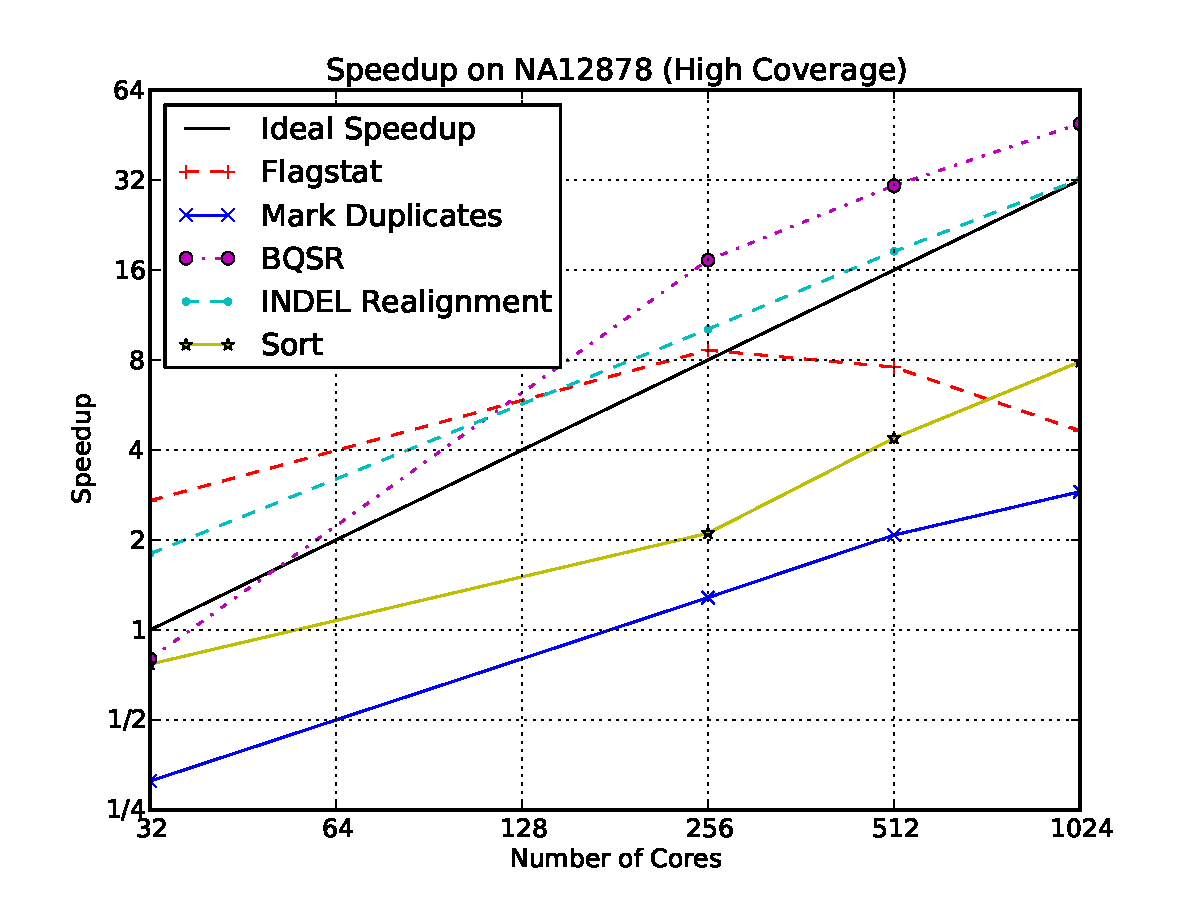
\includegraphics{graphs/speedup_na12878.pdf}
\end{center}
\caption{Speedup on NA12878}
\label{fig:speedup}
\end{figure}

When testing on NA12878, we achieve near-linear speedup out through 1024 cores using 128
\texttt{r3.2xlarge} nodes. In this test, our performance is limited by several factors:

\begin{itemize}
\item Although columnar stores have very high read performance, they have poor write performance. Our
tests exaggerate the penalty of poor write performance since we write the same amount of data as we read. In a typical
variant calling pipeline, the input will be a large read file, but the pipeline's output will be a
variant call file that is approximately two orders of magnitude smaller. Since the amount of data written is much smaller,
the penalty of the reduced write performance is decreased. In practice, we also use in-memory caching to chain stages
together. This amortizes write time across several stages of computation.
\item Additionally, for large clusters, straggler elimination is an issue. However, we have made optimizations to
both the duplicate marking and INDEL realignment code to eliminate stragglers by randomly
rebalancing reads that are unmapped/do not map to a target across partitions.
\end{itemize}

We do note that the performance of Flagstat degrades going from 32 to 128 \texttt{r3.2xlarge} nodes.
Flagstat executes in two minutes on a single node. By increasing the number of machines
we use to execute this query, we increase scheduling overhead, which leads to degraded
performance. When running on the 128 machine cluster, approximately 75\% of the runtime was spent
scheduling and broadcasting the task to be run.

\subsection{Astronomy Workloads}
\label{sec:astro-workloads}

To evaluate the mosaicing application, we use the 2MASS data\footnote{Available from
\url{http://irsa.ipac.caltech.edu/applications/2MASS/IM/}.} and the \texttt{Montage} test case of 3x3 degree
mosaicing with Galaxy m101 as the center. The tile mosaicing phase converts 1.5~GB of input data into a
1.2~GB aggregated output file. We compare the \texttt{Spark-mAdd} performance against the HPC styled
MPI-based parallel implementation from \texttt{Montage} v3.3 (\texttt{MPI-mAdd}). We
performed the test on 1, 4, and 16 Amazon \texttt{c3.8xlarge} instances. We chose the \texttt{c3.8xlarge} instances
for this test because they provided HPC-optimized networking, which is a prerequisite for good MPI performance.
We use \texttt{OrangeFS} v2.8.8---a successor of \texttt{PVFS}~\cite{PVFS}---as the shared file system when running
\texttt{MPI-mAdd}. All 32 cores on each instance are used for both \texttt{Spark-mAdd} and \texttt{MPI-mAdd}.

\begin{figure}[h]
\begin{center}
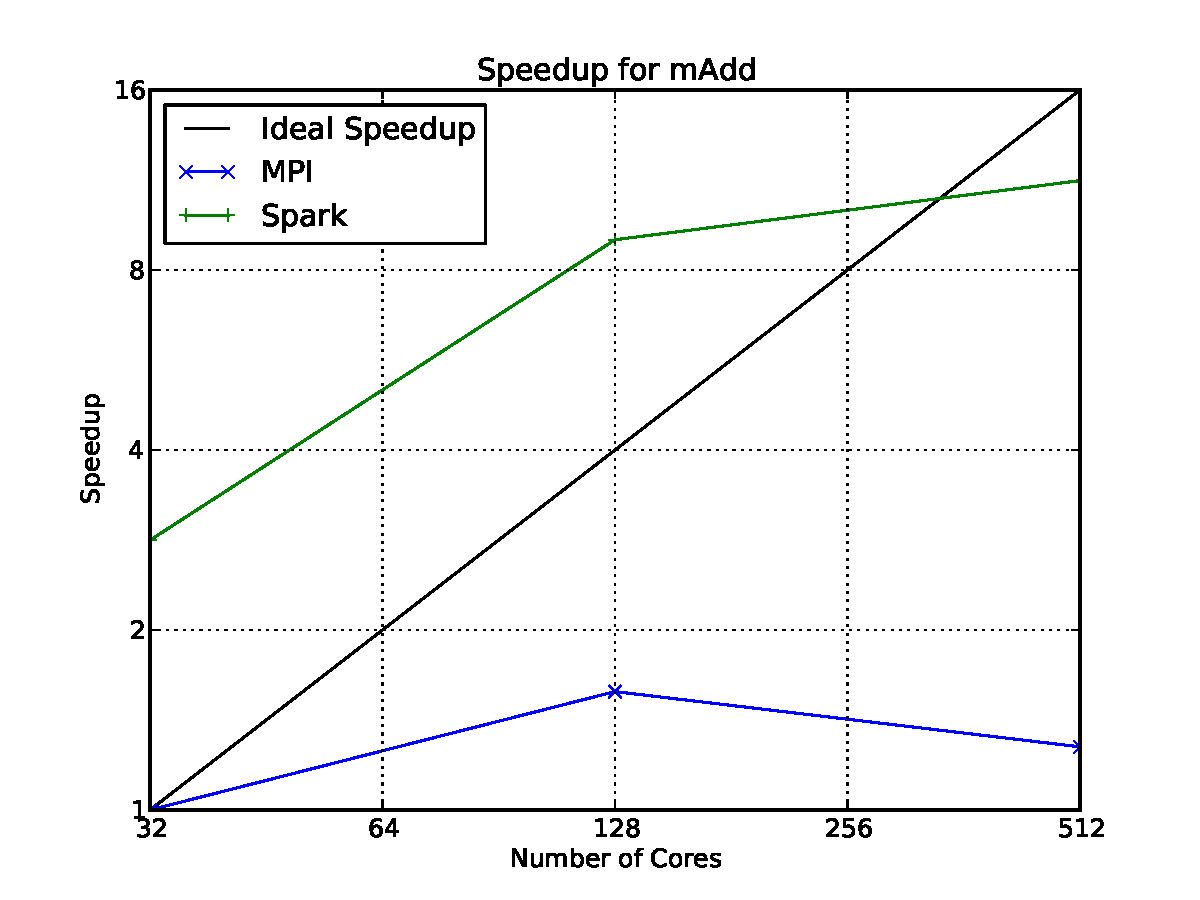
\includegraphics{graphs/speedup_madd.pdf}
\end{center}
\caption{Speedup when running \textit{mAdd} using MPI and Spark}
\label{fig:madd-speedup}
\end{figure}

As shown in Figure~\ref{fig:madd-speedup}, \texttt{Spark-mAdd} runs 2.8x, 5.7x, 8.9x faster than
\texttt{MPImAdd} on 1, 4, and 16 instances. In the single machine case, \texttt{MPI-mAdd} achieves a cost of \$0.17 per
analysis. \texttt{Spark-mAdd} costs \$0.06 to run on a single instance, which is a $2.8\times$ improvement in
cost. \texttt{Spark-mAdd} is still cheaper than \texttt{MPI-mAdd} by a factor of $2.2\times$ when running on four
nodes. \texttt{Spark-mAdd} is only more expensive than a single node of \texttt{MPI-mAdd} when running on 16
nodes, and even then is only 40\% more expensive than the lowest cost \texttt{MPI-mAdd} run while providing a
$8.9\times$ performance improvement over the fastest \texttt{MPI-mAdd} run.

The performance improvement is caused by multiple factors. We are able to reduce the amount of I/O performed,
while also reducing contention in the I/O system and improving data locality. By denormalizing the metadata into
our data schema, we are able to combine the metadata processing stage with the mAdd stage. This combination
allows us to only load the input dataset a single time. \texttt{Parquet} also compresses the input and output data, which
reduces the volume of I/O performed. Additionally, the MPI implementation is bound by contention when trying to write
all output to a single file in a shared file system, while \texttt{Parquet} writes output files into \texttt{HDFS} in a
contention free manner. Finally, \texttt{Spark} allows the computation to benefit from data locality, while MPI distributes
the computation across the available resources without optimizing for data placement.

While the dataset used is a small dataset, larger datasets are commonplace. For example, the Large Synoptic
Survey Telescope~(LSST, \cite{lsst2008}) has been used to collect terabyte sized datasets~\cite{moyers13}. In
future work, we plan to tackle these very large astronomy datasets using our framework.

\subsection{Column Store Performance}
\label{sec:column-store-perf}

Earlier in this paper, we motivated the use of a column store as it would allow us to better push processing to
the data. Specifically, we can use predicate pushdown and projections to minimize the amount of I/O that we
perform. Additionally, column stores provide compressed storage and allow us to minimize both the required
I/O bandwidth and space on disk. In this section, we look at the read performance and compression achieved by
using a columnar store. We will not look extensively at write performance; for genomic
data, write performance is not a bottleneck because our workflow computes a summarization of a large
dataset. As a result, our output dataset tends to be O(100 MB) while our input dataset is in the range of
O(10 GB)--O(100GB).

\subsubsection{Compression}
\label{sec:compression}

The \texttt{Parquet} columnar store~\cite{parquet} supports several compression features. Beyond block-level
compression, \texttt{Parquet} supports run length encoding for repeated values, dictionary encoding, and delta
encoding. Currently, we make use of run length encoding to compress highly repeated metadata value,
and dictionary encoding to compress fields that can take a limited range of values. Dictionary encoding provides
substantial improvements for genomic data; specifically, the majority of genomic sequence data can be
represented with three bits per base.\footnote{Although DNA only contains four bases (A, C, G, and T),
\emph{sequenced} DNA uses disambiguation codes to indicate that a base was read in error. As a result, we
cannot achieve the ideal two-bits per base.} Three bits are an improvement over our in-memory string representation
that allocates a byte per base.

Table~\ref{tab:genomic-compression} shows the compression we achieve on the \texttt{NA12878}
and \texttt{HG00096} human genome sequencing samples~(datasets are described in
Appendix~\ref{sec:experimental-setup}). We compare against the GZIP compressed \texttt{BAM}~\cite{li09} format, and
the \texttt{CRAM} format~\cite{fritz11}. We achieve approximately a $1.25\times$ improvement in storage. This is not as
impressive as the result achieved by the \texttt{CRAM} project, but \texttt{CRAM} applies genome-specific compression
techniques that make use of the read alignment. Specifically, \texttt{CRAM} only stores the read bases that \emph{do
not} appear in the reference genome. As we only expect a genomic variant at one in every 1000 bases, and a read error 
at one in every 50 bases, this allows them to achieve significant compression of the sequenced bases. Additionally,
\texttt{CRAM} applies lossy compression to quality scores. This compression approach is significant, as quality scores
are 60\% of the data stored on disk in the \texttt{ADAM}/\texttt{Parquet} format.

\begin{table}[h]
\caption{Genomic Data Compression}
\label{tab:genomic-compression}
\begin{center}
\begin{tabular}{ l c c }
\hline
\multicolumn{3}{c}{\bf \texttt{NA12878}} \\
\bf Format & \bf Size & \bf Compression \\
\hline
\hline
GZIP BAM & 234 GB & --- \\
CRAM & 112 GB & 2.08$\times$ \\
Parquet & 185 GB & 1.26$\times$ \\
\hline
\multicolumn{3}{c}{\bf \texttt{HG00096}} \\
\bf Format & \bf Size & \bf Compression \\
\hline
\hline
GZIP BAM & 14.5 GB & --- \\
CRAM & 3.6 GB & 4.83$\times$ \\
Parquet & 11.4 GB & 1.27$\times$ \\
\hline
\end{tabular}
\end{center}
\end{table}

The astronomy datasets achieve higher compression ratios. Table~\ref{tab:astro-compression} compares
our storage system against the legacy \texttt{FITS}~\cite{wells81} format. We measured the aggregate compression
of the image files provided as input to our system, and the compression of our pipeline output.

\begin{table}[h]
\caption{Astronomy Data Compression}
\label{tab:astro-compression}
\begin{center}
\begin{tabular}{ l c c }
\hline
\multicolumn{3}{c}{\bf Input Dataset} \\
\bf Format & \bf Size & \bf Compression \\
\hline
\hline
FITS & 1.5 GB & --- \\
Parquet & 0.55 GB & 2.75$\times$ \\
\hline
\multicolumn{3}{c}{\bf Output Dataset} \\
\bf Format & \bf Size & \bf Compression \\
\hline
\hline
FITS & 1.2 GB & --- \\
Parquet & 0.88 GB & 1.35$\times$ \\
\hline
\end{tabular}
\end{center}
\end{table}

For genomic datasets, our compression is limited by the sequence and base quality fields, which respectively
account for approximately 30\% and 60\% of the space spent on disk. Quality scores are difficult to compress
because they are high entropy. We are currently looking into computational strategies to address this problem;
specifically, we are working to probabilistically estimate the quality scores without having observed quality
scores. This estimation would be performed via a process that is similar to the base quality score recalibration
algorithm presented earlier in this paper.

\subsubsection{Horizontal Scalability}
\label{sec:horizontal-scalability}

The representation \texttt{Parquet} uses to store data to disk is optimized for horizontal scalability in several ways.
Specifically, \texttt{Parquet} is implemented as a hybrid row/column store where the whole set of records in a dataset
are partitioned into row groups that are then serialized in a columnar layout. This partitioning provides us with two
additional benefits:

\begin{enumerate}
\item We are able to perform parallel access to \texttt{Parquet} row groups without consulting metadata or checking for
a file split.
\item \texttt{Parquet} achieves very even balance across partitions. On the \texttt{HG00096} dataset, the average
partition size was 105 MB with a standard deviation of 7.4 MB. Out of the 116 partitions in the file, there is only
one partition whose size is not between 105--110MB.
\end{enumerate}

\texttt{Parquet}'s approach is preferable when compared to \linebreak \texttt{Hadoop-BAM}~\cite{niemenmaa12}, a
project that supports the direct usage of legacy \texttt{BAM} files in \texttt{Hadoop}. \texttt{Hadoop-BAM} must pick splits,
which adds non-trivial overhead. Additionally, once \texttt{Hadoop-BAM} has picked a split, there is no guarantee that the
split is well placed. It is only guaranteed that the split position will not cause a functional error. Finally, although
\texttt{BAM} metadata is centralized, \texttt{Hadoop-BAM} punts on metadata distribution, and users must manually
broadcast the metadata.

\subsubsection{Projection and Predicate Performance}
\label{sec:projection-predicate-performance}

We use the Flagstat workload to evaluate the performance of predicates and projections in \texttt{Parquet}.
We define three projections and four predicates, and test all of these combinations. In addition to projecting the
full schema~(see Appendix~\ref{sec:genomics-schema}), we also use the following two projections:

\begin{enumerate}
\item We project the read sequence and all of the flags (40\% of data on disk).
\item We only project the flags (10\% of data on disk).
\end{enumerate}

Beyond the null predicate (which passes every record), we evaluate the following three predicates:

\begin{enumerate}
\item We pass only uniquely mapped reads (99.06\% of reads).
\item We pass only the first pair in a paired end read (50\% of reads, see~\S\ref{sec:genomics-pipeline} for definition of
``paired end'').
\item We pass only \emph{un}mapped reads (0.94\% of reads).
\end{enumerate}

\begin{table}[h]
\caption{Predicate/Projection Speedups}
\label{tab:ppp}
\begin{center}
\begin{tabular}{ l | c c c c }
\hline
& 0 & 1 & 2 \\
\hline
\hline
0 & --- & 1.7 & 1.9 \\
1 & 1.0 & 1.7 & 1.7 \\
2 & 1.3 & 2.2 & 2.6 \\
3 & 1.8 & 3.3 & 4.4 \\
\hline
\end{tabular}
\end{center}
\end{table}

Table~\ref{tab:ppp} documents the speedup we achieve by combining predicate pushdown and projections. Projections
are arranged in the columns of the table while predicates are assigned to rows. We achieve a $1.7\times$ speedup by
moving to a projection that eliminates the deserialization of our most complex field~(the quality scores that consume
60\% of space on disk), while we only get a $1.3\times$ performance improvement when running a predicate that
filters 50\% of records. This difference can be partially attributed to overhead from predicate pushdown; we must first
deserialize a column, process the filter, and then read all records who passed the pushdown filter. If we did not perform
this step, we would be able to do a straight scan over all of the data in each partition.

\section{Discussion and Future Work}
\label{sec:discussion-future-work}

Similar to what we propose, the \texttt{Thunder} system was developed as a novel map-reduce-based system for
processing terabytes of neuroscience imaging data~\cite{freeman14}. \texttt{Thunder} performs a largely statistical
workload, and the significant tasks in terms of execution time are clustering and regression. The system is
constructed using \texttt{Spark} and Python and is designed to process datasets larger than 4 TB, and leverages
significant functionality from the \texttt{MLI}/\texttt{MLLib} libraries~\cite{sparks13}. \texttt{Thunder} uses \texttt{Spark}'s
filtering primitives to allow scientists to cut problems into subproblems. This slicing and dicing is a common trend across
scientific analyses, and is one of the reasons that we advocate for the use of a columnar store with efficient predicate
pushdown.

There has also been work to optimize map-reduce systems for processing geospatial data. Significant
projects include \texttt{SpatialHadoop}~\cite{eldawy15} and \texttt{Hadoop-GIS}~\cite{aji13}. These projects have
focused on indexing strategies that can accelerate range queries against spatial data and improve work balance for
map-reduce tasks run in \texttt{Hadoop} on spatial data. These approaches are similar to the region join that we
propose in~\S\ref{sec:coordinate-system-joins}, but restricted to geospatial and imaging data.

Our genomics work leverages columnar storage to improve performance and compression of data on disk,
with special emphasis on repetitive fields that can be run length encoded~(RLE). While this improves
disk performance, it has the side effect of making data consume significantly more space in memory
than on disk. We are currently investigating techniques that leverage the immutability of data in our
applications to reduce memory consumption and have modified \texttt{Parquet}'s deserialization codec. For
every value that is RLE'd, we allocate the value once in memory and share the value across all records which
contained that value. This allocation pattern enables denormalizing repeated metadata.

It is worth noting that there are many significant scientific applications (such as genome
assembly) that are expressed as traversal over graphs. Recent work by Simpson et al~(\texttt{ABySS},
\cite{simpson09}) and Georganas et al~\cite{georganas14} has focused on using MPI
or Unified Parallel C~(UPC) to implement their own distributed graph traversal. Both systems
find that synchronization via message passing is a significant cost. By building our system using \texttt{Spark}, we are
able to leverage the \texttt{GraphX} processing library~\cite{gonzalez14,
xin13}. We are in the process of developing a genome assembler using this library system, and
believe that we can achieve improved performance through careful graph partitioning. This partitioning involves
algorithmic changes to the graph creation and traversal phases to bypass ``knotted'' sections of the graph.

In this paper, we focus on the \texttt{GATK}~\cite{depristo11} as an example of a genome processing pipeline that
needs to be distributed to improve analysis latency and throughput. While the \texttt{GATK} is widely used,
there is significant debate as to whether the expensive methods employed by the \texttt{GATK} are necessary. Several
new ``minimal preprocessing'' based methods such as \texttt{SpeedSeq}~\cite{chiang14} have achieved achieved
results that are comparable to the \texttt{GATK}, while eliminating the computationally expensive BQSR and INDEL
realignment stages. While these approaches do improve throughput, they do not tackle parallelism beyond a single
machine, which will be necessary for analyzing very large cohorts. Additionally, the proponents of ``minimal'' pipelines
frequently validate accuracy on high quality, whole genome sequencing datasets. Since whole genome sequencing
methods contain fewer sources of error than targeted/whole exome sequencing panels, a more comprehensive
evaluation is needed to validate the impact of removing expensive stages.

\section{Conclusion}
\label{sec:conclusion}

In this paper, we have advocated for an architecture for decomposing the implementation of a scientific system, and
then demonstrated how to efficiently implement genomic and astronomy processing pipelines using the open source
\texttt{Avro}, \texttt{Parquet}, and \texttt{Spark} systems~\cite{avro, parquet, zaharia10}. We have identified common
characteristics across scientific systems, like the need to run queries that touch slices of datasets and the need
for fast access to metadata. We then enforced data independence through a layering model that uses a schema
as the ``narrow waist'' of the stack, and used optimizations to make common, coordinate-based processing
fast. By using Parquet, a modern columnar store, we use predicates and projections to minimize I/O, and
denormalize our schemas to improve the performance of accessing metadata.

By rethinking the architecture of scientific data management systems, we have been able to achieve parity on single
node systems, while providing linear strong scaling out to 128 nodes. By making it easy to scale scientific analyses
across multiple commodity machines, we enable the use of smaller, less expensive computers, leading to a 63\% cost
improvement and a 28$\times$ improvement in read preprocessing pipeline latency. On the astronomy workload, we
achieve speedup between 2.8--$8.9\times$ speedup over the current
best MPI-based solution at various scales. By applying our techniques to both astronomy and genomics, we have
demonstrated that the techniques are applicable to both traditional matrix-based scientific computing, as well as novel
scientific areas that have less structured data.

\section{Acknowledgements}

This research is supported in part by NSF CISE Expeditions Award CCF-1139158, LBNL Award 7076018, and DARPA XData Award FA8750-12-2-0331, NIH BD2K Award \linebreak 1-U54HG007990-01, NIH Cancer Cloud Pilot Award \linebreak HHSN261201400006C and gifts from Amazon Web Services, Google, SAP,  The Thomas and Stacey Siebel Foundation, Adatao, Adobe, Apple, Inc., Blue Goji, Bosch, C3Energy, Cisco, Cray, Cloudera, EMC, Ericsson, Facebook, Guavus, Huawei, Intel, Microsoft, NetApp, Pivotal, Samsung, Splunk, Virdata, VMware, and Yahoo!. Author FAN is supported by a National Science Foundation Graduate Research Fellowship.

We would also like to thank our colleagues who have provided feedback and engineering effort to the \texttt{ADAM} system, including Andr\'{e} Schumacher, Christopher Hartl, Karen Feng, Eric Tu, Kristal Curtis, Taylor Sittler, Neal Sidhwaney, Ryan Williams, Ravi Pandya, and the UCSC Genome Bioinformatics group. As \texttt{ADAM} is an open source project, we also would like to thank the community members who have contributed code and use cases to the project, and would especially like to thank Neil Ferguson, Andy Petrella, Xavier Tordior, and Michael Heuer. Additionally, the authors would like to thank the anonymous reviewers and our shepherd, Ken Yocum, for their helpful commentary on this paper.

\balance

\clearpage

\appendix

\bibliographystyle{abbrv}
\bibliography{adam}

\section{Schemas}
\label{sec:schema}

Here, we present the schemas that we have used for these two systems. To clarify the schemas, we
have grouped our fields into a simpler logical schema ordering, and we have also removed the \texttt{Avro} syntactic
sugar used to ensure that all fields are nullable, which is required to enable arbitrary
projections. These schemas are implemented using \texttt{Avro}~\cite{avro}, and data is stored to disk via
\texttt{Parquet}~\cite{parquet}. In-memory \linebreak (de-)serialization is provided via a custom wrapper around
\texttt{Avro}'s serialization framework.

\subsection{Genomics Schema}
\label{sec:genomics-schema}

The schema used for storing genomic short read data is described below:

\begin{lstlisting}
record AlignmentRecord {
  /** Alignment position and quality */
  Contig contig;
  long start;
  long oldPosition;
  long end;

  /** read ID, sequence, and quality */
  string readName;
  string sequence;
  string qual;
  
  /** alignment details */
  string cigar;
  string oldCigar;
  int mapq;
  int basesTrimmedFromStart;
  int basesTrimmedFromEnd;
  boolean readNegativeStrand;
  boolean mateNegativeStrand;
  boolean primaryAlignment;
  boolean secondaryAlignment;
  boolean supplementaryAlignment;
  string mismatchingPositions;
  string origQual;

  /** Read status flags */
  boolean readPaired;
  boolean properPair;
  boolean readMapped;
  boolean mateMapped;
  boolean firstOfPair;
  boolean secondOfPair;
  boolean failedVendorQualityChecks;
  boolean duplicateRead;

  /** optional attributes */
  string attributes;

  /** record group metadata */
  string recordGroupName;
  string recordGroupSequencingCenter;
  string recordGroupDescription;
  long recordGroupRunDateEpoch;
  string recordGroupFlowOrder;
  string recordGroupKeySequence;
  string recordGroupLibrary;
  int recordGroupPredictedMedianInsertSize;
  string recordGroupPlatform;
  string recordGroupPlatformUnit;
  string recordGroupSample;

  /** Mate pair alignment information */
  long mateAlignmentStart;
  long mateAlignmentEnd;
  Contig mateContig;
}
\end{lstlisting}

All of the metadata from the sequencing run and prior processing steps are packed into the record
group metadata fields. The program information describes the processing lineage of the sample and
is expected to be uniform across all records, thus it compresses extremely well. The record group
information is not guaranteed to be uniform across all records, but there are a limited number number
of record groups per sequencing dataset. This
metadata is string heavy, which makes proper deserialization from disk important. Although the
information consumes less than 5\% of space on disk, a poor deserializer implementation may replicate
a string per field per record.

We have defined common projections and predicates to operate on these records. For
example, tools that perform quality control for sequenced data commonly only access the read status flags.
Additionally, it is common to run predicates on the read position,
or whether the read is mapped or not. We have implemented code that allows us to apply these predicates to legacy
datasets that do not support
direct predicate pushdown. On legacy data, we only get the functionality of the predicate, not the
performance improvement.

\subsection{Astronomy Schema}
\label{sec:astronomy-schema}

We use the following schema for storing astronomy pixel values:

\begin{lstlisting}
record PixelValue {
  /** pixel position */
  int xPos;
  int yPos;
  
  /** pixel value */
  float value;
  
  /** file metadata */
  int start;
  int end;
  int offset;
  int height;
}
\end{lstlisting}

This schema is derived from the legacy Flexible Image Transport System~(\texttt{FITS},~\cite{wells81}), which
defines an interchange format for astronomy images. During the \texttt{mAdd} processing kernel
described in~\S\ref{sec:astro-workloads}, we access the file metadata from each pixel. In current systems,
metadata access becomes a significant performance bottleneck as we are performing metadata access
across thousands of files~\cite{zhang13}.

\section{Convex-Hull Finding}
\label{sec:convex-hull}

A frequent pattern in our application is identifying the maximal convex hulls across sets of regions. For
a set $R$ of regions, we define a maximal convex hull as the largest region $\hat{r}$ that satisfies the
following properties:

\begin{align}
\label{eqn:convexity-constraint}
\hat{r} &= \cup_{r_i \in \hat{R}} r_i \\
\hat{r} \cap r_i &\ne \emptyset, \forall r_i \in \hat{R} \\
\hat{R} &\subset R
\end{align}

In our problem, we seek to find all of the maximal convex hulls, given a set of regions. For genomics, the
convexity constraint described by \eqref{eqn:convexity-constraint} is trivial to check: specifically, the
genome is assembled out of reference sequences that define disparate 1-D coordinate spaces. If two regions exist
on different sequences, they are known not to overlap. If two regions are from a single single, we simply check to see if
they overlap in that 1-D coordinate plane. We define the data-parallel Algorithm~\ref{alg:parallel-convex-hull} to find
the maximal convex hulls that describe a genomic dataset.

\begin{algorithm}[t]
\caption{Find Convex Hulls in Parallel}
\label{alg:parallel-convex-hull}
\begin{algorithmic}
\STATE $data \leftarrow$ input dataset
\STATE $regions \leftarrow data$.map($data \Rightarrow $generateTarget($data$))
\STATE $regions \leftarrow regions$.sort()
\STATE $hulls \leftarrow regions$.fold($r_1, r_2 \Rightarrow$ mergeTargetSets($r_1, r_2$))
\RETURN $hulls$
\end{algorithmic}
\end{algorithm}

The \texttt{generateTarget} function projects each datapoint into a Red-Black tree which contains a
single region. The performance of the fold depends on the efficiency of the merge function. We achieve
efficient merges with the tail-call recursive \texttt{mergeTargetSets} function which is described in
algorithm~\ref{alg:join-targets}.

\begin{algorithm}[b]
\caption{Merge Hull Sets}
\label{alg:join-targets}
\begin{algorithmic}
\STATE $first \leftarrow$ first target set to merge
\STATE $second \leftarrow$ second target set to merge
\REQUIRE $first$ and $second$ are sorted
\IF{$first = \emptyset \wedge second = \emptyset$}
\RETURN $\emptyset$
\ELSIF{$first = \emptyset$}
\RETURN $second$
\ELSIF{$second = \emptyset$}
\RETURN $first$
\ELSE
\IF{last($first$) $\cap$ head($second$) $= \emptyset$}
\RETURN $first$ + $second$
\ELSE
\STATE $mergeItem \leftarrow$ (last($first$) $\cup$ head($second$))
\STATE $mergeSet \leftarrow$ allButLast($first$) $\cup mergeItem$
\STATE $trimSecond \leftarrow$ allButFirst($second$)
\RETURN mergeTargetSets($mergeSet$, $trimSecond$)
\ENDIF
\ENDIF
\end{algorithmic}
\end{algorithm}

For a region join~(see~\S\ref{sec:coordinate-system-joins}), we can use the maximal convex hull
set to define partitioning for the join. Alternatively, for INDEL realignment~(see~\S\ref{sec:genomics-pipeline}),
we use this set as an index for mapping reads directly to targets.

\section{Availability}
\label{sec:availability}

The source code of both \texttt{ADAM} and \texttt{SparkMontage}, and our schemas are released under the Apache 2
license. \texttt{ADAM} is available at \url{https://www.github.com/bigdatagenomics/adam}, and \texttt{SparkMontage}
is at \url{https://www.github.com/zhaozhang/SparkMontage}. \texttt{ADAM}'s schemas are available at
\url{https://www.github.com/bigdatagenomics/bdg-formats}. \linebreak \texttt{ADAM} is released via the Apache Maven
Central repository, with the following dependencies:

\begin{verbatim}


<dependency>
  <groupId>org.bdgenomics.bdg-formats</groupId>
  <artifactId>bdg-formats</artifactId>
</dependency>
<dependency>
  <groupId>org.bdgenomics.adam</groupId>
  <artifactId>adam-distribution</artifactId>
</dependency>
\end{verbatim}

As of the final submission of this paper, the latest releases of \texttt{ADAM} and \texttt{bdg-formats} were 0.16.0 and 0.4.0.

\section{Experimental Setup}
\label{sec:experimental-setup}

The datasets and scripts used in the genomics experiments in this paper are all freely available online
and can be used to reproduce our analyses. We made use of the \texttt{NA12878} and \texttt{HG00096}
datasets from the 1000 Genome project when running our experiments~\cite{siva08}. These two datasets
are available from either of the 1000 Genome project anonymous FTP servers
(\url{ftp.1000genomes.ebi.ac.uk/vol1/ftp/} or \url{ftp://ftp-trace.ncbi.nih.gov/1000genomes/ftp}), and are
also hosted publicly on Amazon S3 (\url{s3://1000genomes}). These datasets reside at the following
locations on those servers:

\begin{itemize}
\item \texttt{NA12878}: \texttt{data/NA12878/high\_coverage\_alignment/}
\item \texttt{HG00096}: \texttt{data/HG00096/alignment/}
\end{itemize}

Our experiments were run on Amazon EC2 using either default or publicly available machine images.
Scripts used to run the experiments are available under the Apache 2 license from the \texttt{bdg-recipes} 
repository, at \url{https://www.github.com/bigdatagenomics/bdg-recipes}. Our experimental scripts
assemble \texttt{ADAM} release 0.16.0, \texttt{GATK} release 3.3~\cite{depristo11}, \texttt{Sambamba}'s docker
image~\cite{tarasov15}, \texttt{SAMBLASTER} 0.1.21~\cite{faust14}, and \texttt{Picard}
\texttt{b2a94f7}~\cite{picard}. These were the latest versions of these tools at the time of final submission. These
evaluation scripts run and time the experiments listed in this paper.

\balance

\end{document}
